\documentclass[aps,prl,twocolumn,superscriptaddress,showpacs,longbibliography]{revtex4-1}
\usepackage{graphicx}
\usepackage{amsfonts}
\usepackage{verbatim}
\usepackage{amssymb}
\usepackage{color}
\usepackage{amsmath} % or simply amstext
\usepackage{hyperref}
\hypersetup{colorlinks = true, urlcolor = blue, linkcolor = blue, citecolor = blue}




%%%% begin of New definition of commands %%%%


\newcommand{\bs}{\boldsymbol}
\newcommand{\angstrom}{\text{\normalfont\AA}}


\newcommand{\su}{\uparrow} 
\newcommand{\sd}{\downarrow} 
\newcommand{\bpm}{\begin{pmatrix}}
\newcommand{\epm}{\end{pmatrix}}

\newcommand{\tn}{\tau_0}
\newcommand{\tx}{\tau_x}
\newcommand{\ty}{\tau_y}
\newcommand{\tz}{\tau_z}
\newcommand{\sgn}{\sigma_0}
\newcommand{\sgx}{\sigma_x}
\newcommand{\sgy}{\sigma_y}
\newcommand{\sgz}{\sigma_z}
\newcommand{\sn}{s_0}
\newcommand{\sx}{s_x}
\newcommand{\sy}{s_y}
\newcommand{\sz}{s_z}

\newcommand{\nn}{\nonumber \\} 
\newcommand{\tp}{ ^{\intercal} }
\newcommand{\dg}{^{\dagger}}
\newcommand{\hc}{\rm{H.c.}}
\newcommand{\half}{\frac{1}{2}}
\newcommand{\br}{\bold{r}}
\newcommand{\bx}{\bold{x}}
\newcommand{\bk}{\bold{k}}
\newcommand{\bp}{\bold{p}}
\newcommand{\bq}{\bold{q}}
\newcommand{\tro}{\mathcal{T}}

\newcommand{\nb}{\bar{n}}
\DeclareMathOperator\arcsinh{arcsinh}

%%%% end of New definition of commands %%%%


\begin{document}

\title{Magnetic proximity effect at superconductor-ferromagnet interfaces}

\author{Chun-Xiao Liu}
\email{Electronic address: chunxiaoliu62@gmail.com}
\affiliation{Qutech and Kavli Institute of Nanoscience, Delft University of Technology, Delft 2600 GA, The Netherlands.}

\author{Haining Pan}
\affiliation{Condensed Matter Theory Center and Joint Quantum Institute,
Department of Physics, University of Maryland, College Park, Maryland 20742, USA}

\date{\today}

\begin{abstract}
Motivated by the recent experimental progress in ferromagnetic hybrid nanowires, we study the magnetic proximity effect in a mesoscopic superconductor-ferromagnet bilayer.
We adopt the method of microscopic model simulation, which treats both materials on equal footing.
By numerically calculating the density of states, band diagram, and wavefunction profiles, we find that in the clean superconductor limit, the induced exchange coupling depends sensitively on the momenta of a particular state.
In particular, a large momentum parallel to the interface would strongly suppress the induced coupling by renormalizing the penetration length in the ferromagnet.
However, such a sensitivity would be averaged out in the presence of a disorder potential in the superconductor.
We also show the dependence of the induced coupling on other physical and geometrical parameters in the system. 
Finally we show a self-consistent treatment of the mean-field superconductivity in the presence of both disorder and ferromagnetism.
\end{abstract}



\maketitle


\emph{Introduction.}--Superconductivity and spin splitting are two indispensable ingredients for engineering topological superconductivity in spin-orbit coupled semiconducting materials.
Usually, spin splitting is induced by a magnetic field applied in large-$g$-factor semiconductors.
Recently, zero-field signatures of Majoranas in tunnel spectroscopy have also been observed in InAs/EuS/Al hybrid nanowires, for which the spin splitting is induced by a ferromagnetic insulator.
In particular, such signatures appear only when the Al and EuS layers overlap, indicating the important interplay between superconductivity (S) and ferromagnet (F) in these topological quantum devices.


Several works have theoretically investigated the magnetic proximity effect between S and F.
In the clean S limit, Ref.~\cite{Langbehn2020Topological} found that the induced coupling is state-dependent and that the normal-superconductor transition is continuous as the strength of the exchange coupling goes through the critical value.
By contrast, in Ref.~\cite{Khindanov2020Topological}, the authors considered a diffusive S, and the quasiclassical calculations showed that the effect of F is equivalent to a uniform Zeeman field in S, and that the normal-superconductor transition is of the second order.
Therefore, a gap of understanding remains as for how the electronic properties of the bilayer evolve between the clean and diffusive limits.
What's more, all these works modeled the effect of F as a phenomenological boundary condition on S, and thus little is known about the inverse proximity effect to F, e.g., the renormalization of the penetration length.
Such a knowledge may become crucial when considering a proposal in which the ferromagnet serves as a spin-filtering barrier layer between the semiconductor and the superconductor~\cite{Maiani2021Topological}.



In the current work, we treat superconductivity and ferromagnet on equal footing by using the microscopic tight-binding model, and focus on the magnetic proximity in an S-F bilayer.
We find that the induced exchange coupling depends sensitively on the momenta of a particular state, and that such a sensitivity would be averaged out in the presence of a disorder potential in S.
In particular, the penetration length into F can be renormalized by the kinetic energy parallel to the interface.
We also show the dependence of the induced coupling on all other relevant physical and geometrical parameters in the system. 
Finally a self-consistent calculation of the mean-field superconductivity is performed, exploring the type of normal-superconductor phase transition and the evolution of the pairing and spectral gaps in the presence of disorder and ferromagnetism.








\begin{figure}
\centering
{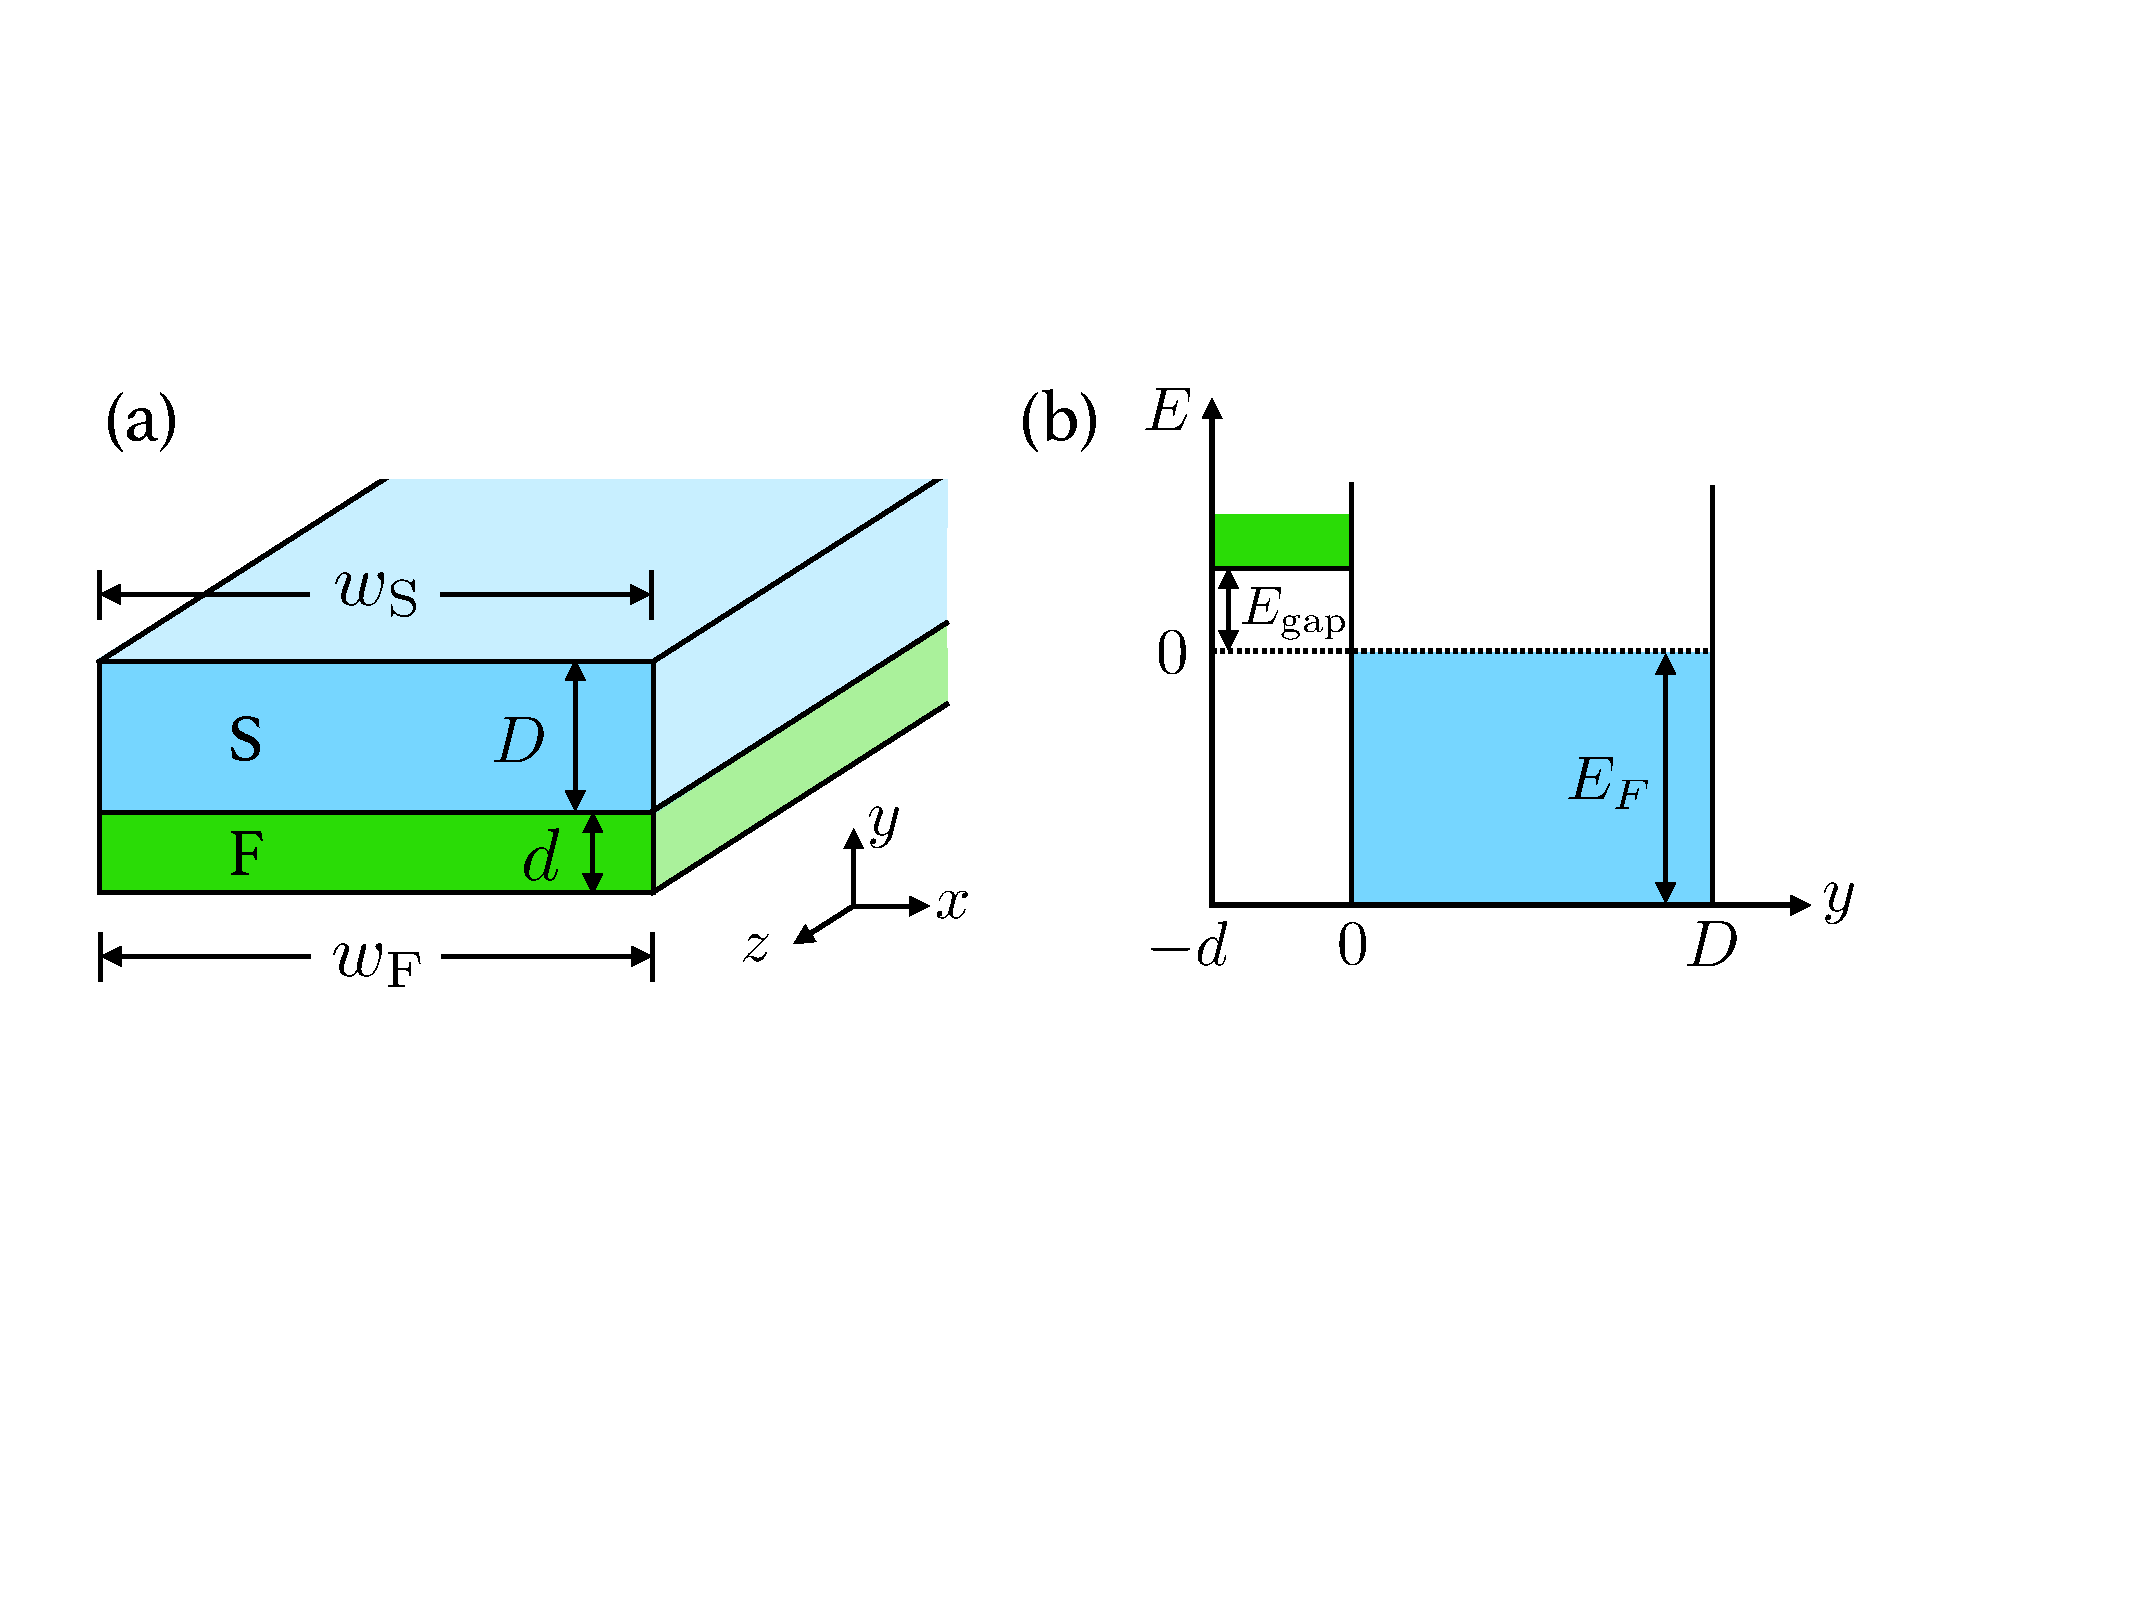
\includegraphics[width = \linewidth]{Fig_1.pdf}}
\caption{(a) Schematic of the superconductor-ferromagnet bilayer model studied in this work. The heterostructure has a rectangular cross section in the $xy$-plane, and translational symmetry along the $z$-axis. (b) Diagram of the conduction-band electrons in the bilayer.}
\label{fig:Fig_1}
\end{figure}








\emph{Model Hamiltonian and method.}--We consider an S-F bilayer, which has a rectangular cross section in the $xy$-plane and translational symmetry along the $z$-axis, as shown in Fig.~\ref{fig:Fig_2}(a).
The S part occupies the region of $0 \leq x \leq w$ and $0 < y \leq D$, and the F layer occupies $0 \leq x \leq w$ and $-d \leq y \leq 0$.
The Bogoliubov Hamiltonian of the heterostructure is
\begin{align}
H_{\text{BdG}} &= \left( \frac{\hbar^2(-\partial^2_x +  k^2_z)}{2 m(y)}  -\frac{\hbar^2}{2} \partial_y \frac{1}{m(y)} \partial_y + E_b(y)   \right) \tau_z \nn
&+ V(x, y) \tau_z + h(y) \sigma_z + \Delta(y) \tau_x,
\label{eq:H_BdG}
\end{align}
where $\sigma_{x,y,z}$ and $\tau_{x,y,z}$ are Pauli matrices acting on the spin and Nambu space, and the basis for $H_{\text{BdG}}$ is $(u_{\su}, u_{\sd}, v_{\sd}, -v_{\su})\tp$. Here $\hbar$ is the Planck constant, $m(y)$ is the effective mass with $m(y>0) = m_{\text{S}}= m_e$ and $m(y \leq 0) = m_{\text{F}}= 0.3~m_e$, with $m_e$ being the electron rest mass, $k_z$ is the wave-vector along the $z$-axis, and $E_b$ is the conduction band edge with $E_b(y>0) = -E_F = -11~$eV and $E_b(y \leq 0) = E_{\text{gap}} = 0.5~$eV. $V(x,y)$ is the disorder potential inside the S region, and we assume that the disorder potential is spatially uncorrelated and obeys an uniform distribution: $ V(x,y) \in [-U_{\text{D}}, U_{\text{D}})$. $h(y \leq 0) = h$  is the strength of the exchange field in F, and $\Delta(y>0) = \Delta_0=0.35~$meV is the pairing potential of S. Note that in the current work, we use the physical parameters of Al and EuS for our S-F bilayer model calculations. 
However, our conclusions are general and do not reply on the precise values of these parameters.





\begin{figure}[t]
\centering
{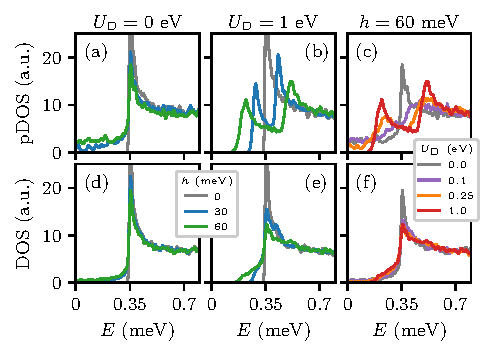
\includegraphics[width = \linewidth]{Fig_2.pdf}}
\caption{Upper panels: partial DOS of the S-F bilayer. (a) and (b) A clean and a disordered S layer for different values of $h$ in F. (c) An S layer for different disorder strengths, with $h$ in F being fixed. Lower panels: total DOS of the S-F bilayer, with the system parameters being identical to the counterparts in the upper panels. }
\label{fig:Fig_2}
\end{figure}


In the numerical calculations, we discretize the BdG Hamiltonian in Eq.~\eqref{eq:H_BdG} into a tight-binding model on a square lattice in the $xy$-plane, and obtain the eigen-energies $E_{n, k_z}$ and the eigen-wavefunctions $[ u_{n, k_z, \su}(x,y), u_{\sd}, v_{\sd}, -v_{\su} ]\tp$ by sparse-matrix diagonalization. The width of the bilayer is 50~nm, and the thickness of the S and F layers are 10~nm and 2~nm, respectively, unless stated otherwise.
The geometry parameters are chosen in accordance with the hybrid devices studied in experiments.
The density of states (DOS) of the system is defined as $\text{DOS}(E) = N^{-1}_{k_z}\sum_{n} \sum_{|k_z| < k_F} \delta(E - E_{n, k_z})$, for which the $k_z$-summation is limited by the Fermi wave-vector $k_F \approx 20~\text{nm}^{-1}$.
Additionally, in order to distinguish the magnetic proximity effects on states with small and large $k_z$, we also define the partial density of states (pDOS) for a partial $k_z$-summation, i.e., $\sum_{|k_z| < k_*}$ with $k_* \approx 3~\text{nm}^{-1} \ll k_F$. The induced exchange coupling for a particular state is $h_{\text{ind}} = \int_{ y \leq 0} d\bold{r} h(\bold{r})( |u_{\su}(\bold{r})|^2 - |u_{\sd}(\bold{r})|^2 + |v_{\sd}(\bold{r})|^2 -  |v_{\su}(\bold{r})|^2 )$, with $\bold{r}=(x,y)$. 
More details of the numerical calculations are in the supplementary material.

\emph{Density of states, band diagram and wavefunctions.}--We first calculate the partial and total DOS of the S-F bilayer.
Figures~\ref{fig:Fig_2}(a) and~\ref{fig:Fig_2}(d) show the DOS for a clean S.
There is a single DOS peak at $E = \Delta_0$ in the absence of exchange coupling in F.
The peak remains there and does not split at finite exchange coupling, with only some softening of the gap.
In contrast, when S is disordered, the single peak at $E = \Delta_0$ splits into two peaks at finite $h$, and the distance of the two split peaks increases with $h$, as shown in Fig.~\ref{fig:Fig_2}(b). 
However, such a clear signature of peak splitting only happens for pDOS.
For the total DOS of a disordered S, the single DOS peak remains at $E = \Delta_0$, and the split peaks observed in pDOS are now smeared and appear as minor kinks in the DOS profiles, as shown in Fig.~\ref{fig:Fig_2}(e).
Figures~\ref{fig:Fig_2}(c) and~\ref{fig:Fig_2}(f) show the evolution of the DOS profiles at fixed $h$ for different strengths of the disorder potential. For pDOS, the single peak at $E=\Delta_0$ is gradually smeared out until two split peaks form below and above the bare gap.
While for total DOS, a stronger strength of disorder potential only lowers the single peak at $E=\Delta_0$ and suppresses the DOS near $E=0$.


%Our DOS calculations indicate that only those small $k_z$ states in a disordered S would share an induced exchange coupling of nearly equal strength, similar to the scenario with an applied Zeeman field in S. 
%In other cases, either in a clean S or including all the Fermi level states, the majority of the states has only negligible induced coupling, and thereby the single DOS peak at $E=\Delta_0$ remains.

\begin{figure}[t]
\centering
{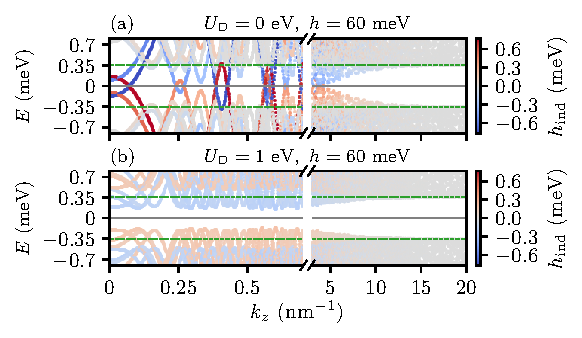
\includegraphics[width = \linewidth]{Fig_3.pdf}}
\caption{Band diagram for the S-F bilayer. (a) Clean S. (b) Disordered S.
Note that the induced exchange coupling varies between different transverse modes in clean S, while is approximately the same in disordered S. In both cases, the induced coupling decreases with increasing $k_z$. }
\label{fig:Fig_3}
\end{figure}


Figure~\ref{fig:Fig_3} shows the band diagram and the induced exchange coupling at $h=60~$meV for the bilayer in clean and dirty S limit.
In the clean limit, the induced coupling $h_{\rm{ind}}$ is state-dependent and ranges from 0 to about $2\Delta_0$ for small $k_z$ states ($k_z < 0.5~\rm{nm}^{-1}$).
In contrast, for dirty S, all the small $k_z$ states share a similar strength of induced coupling.
In both cases, the induced coupling starts to decrease at $k_* \approx 3~\rm{nm}^{-1}$, and the proximity effect almost vanishes for large $k_z$ states ($k_z > 10~\rm{nm}^{-1}$).
A closer examination on the wavefunction profiles, i.e., $ |\psi|^2= \sum_{\sigma=\su,\sd}( |u_{\sigma}|^2  + |v_{\sigma}|^2)$, shows that states with a larger momentum perpendicular to the S-F interface [see Fig.~\ref{fig:Fig_4}(a)] tends to have a stronger induced coupling compared to those with a small transverse momentum [see Fig.~\ref{fig:Fig_4}(b)].
In a disordered S, the wavefunction profile becomes random in space [see Figs.~\ref{fig:Fig_4}(c) and~\ref{fig:Fig_4}(d)], and the penetration length into F decreases with increasing $k_z$[see Fig.~\ref{fig:Fig_4}(f)]












\begin{figure}
\centering
{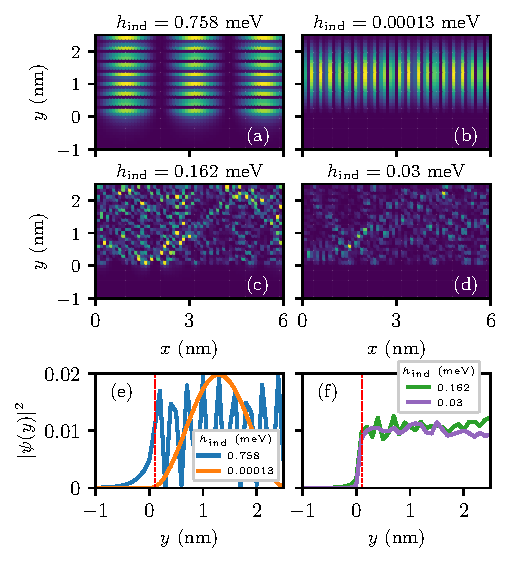
\includegraphics[width = \linewidth]{Fig_4.pdf}}
\caption{Wavefunction profiles of the states near the Fermi level, with $h=60~$meV in F.
The profiles are shown in a selected region of the cross section for clarity of presentation but without loss of generality.
(a) and (b) $U_{\text{D}}=0~$, $k_z=0$.
In a clean S, eigenstates with large (small) momenta normal to the interface have a strong (weak) induced exchange coupling.
(c) $U_{\text{D}}=1~$eV, $k_z=0$.
(d) $U_{\text{D}}=1~$eV, $k_z=10~\text{nm}^{-1}$. 
The wavefunction profile now becomes random in the presence of disorder.
A larger $k_z$ parallel to the interface weakens the magnetic proximity effect.
(e) and (f) Wavefunction profiles $|\psi(y)|^2$ projected along $y$-axis. The red dashed line indicates the S boundary at the interface. In (f), the state with a larger $k_z$ has a shorter penetration length in F.
}
\label{fig:Fig_4}
\end{figure}


\emph{Dependence on other parameters.}--We also study the dependence of the induced exchange coupling on all the relevant physical and device parameters.
Here we focus on a disordered S and $h_{\rm{ind}}$ is averaged over the 60 states near the Fermi level and $|k_z| < 1~\text{nm}^{-1}$.
In Fig.~\ref{fig:Fig_5} we see that $h_{\rm{ind}}$ is proportional to the bare exchange coupling $h$ in F, and decreases monotonically with the insulating gap in F or the thickness of S [see Figs.~\ref{fig:Fig_5}(a), \ref{fig:Fig_5}(b) and ~\ref{fig:Fig_5}(d)].
The induced coupling $h_{\rm{ind}}$ generally increases with the size of F, and will saturate once the thickness $d$ is large enough or when F is wider than S [see Figs.~\ref{fig:Fig_5}(e) and ~\ref{fig:Fig_5}(f)].
In Fig.~\ref{fig:Fig_5}(c), we consider a magnetic domain in F, with the exchange field pointing in the $+z$ ($-z$) direction to the left (right) of the domain wall. 
That is, the exchange field profile is $h(\bold{r}) = h\theta(x_{\rm{DW}} - x) - h\theta(x - x_{\rm{DW}})$ with $\theta(x)$ being the heaviside step-wise function.
The result shows that the induced coupling is the maximum when a single domain occupies the whole F, and is reduced to the minimum when $+z$ and $-z$ domains are of the same size.


\begin{figure}
\centering
{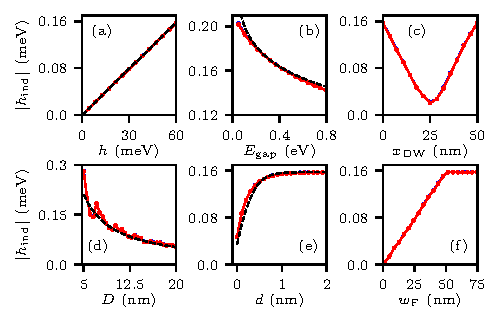
\includegraphics[width = \linewidth]{Fig_5.pdf}}
\caption{Dotted lines: Numerically calculated $h_{\rm{ind}}$ as a function of (a) exchange coupling in F, (b) insulating gap in F, (c) position of the magnetic domain wall in F, (d) thickness of S, (e) thickness of F, and (f) width of F. Note that the amplitudes are essentially identical for $h_{\text{ind}} > 0$ (red) and $h_{\text{ind}} < 0$ (blue) .
Dashed lines: Analytic estimations. }
\label{fig:Fig_5}
\end{figure}



\emph{Analytic approach.}--In order to understand the numerical results, we use the wave-function approach to analyze the magnetic proximity effect in the bilayer. Since superconductivity is not essential for the magnetic proximity effect and the width of the bilayer is much larger than the thickness, here we consider a planar normal metal-ferromagnet bilayer, focusing on the eigenstates at the Fermi level, that is,
\begin{align}
\left( -\frac{\hbar^2}{2} \partial_y \frac{1}{m(y)} \partial_y + \frac{\hbar^2k^2_{\parallel}}{2 m(y)} + E_b(y)   \right) \phi(y) = 0,
\end{align}
with $k^2_{\parallel} = k^2_x + k^2_z$ being the momentum parallel to the interface, and $\hbar^2(k^2_y + k^2_{\parallel})/2m_{\rm{S}} \approx E_F$. We neglect the spin degree of freedom because spin polarization is a conserved quantity in this problem. By matching the wavefunction and its first-order derivative at the interface ($y=0$) and applying the boundary condition $ \phi(D) = \phi(-d) =0$, we obtain
\begin{align}
\psi(y) = \left\{ 
\begin{array}{ll}   \sin (k_y(y-D))  \quad  \text{for }  y>0,\\
   \frac{ \sin (k_y D)}{ e^{-2d/\lambda} - 1} \left( e^{y/\lambda} -  e^{-(y+2d)/\lambda} \right)  \text{for }  y \leq 0,
\end{array}\right.
\end{align}
up to a normalization constant. Here $\lambda$ is the renormalized penetration length
\begin{align}
\lambda = \frac{1}{\sqrt{\lambda^{-2}_0 + k^2_{\parallel} }}
\label{eq:lambda}
\end{align}
with $\lambda^{-1}_0 =   \sqrt{2m_{\rm{F}}E_{\text{gap}}} / \hbar$ being the bare penetration length. The allowed values of momentum $k_y$ normal to the interface is determined by the transcendental equation
\begin{align}
-k_y \lambda \cdot \frac{m_{\rm{F}}}{m_{\rm{S}}} \cdot  \tanh (d/\lambda) = \tan (k_y D).
\label{eq:trans}
\end{align}
The induced exchange coupling for the eigenstate is
\begin{align}
h_{\rm{ind}} =  \frac{ h \int^0_{-d} dy |\phi(y)|^2}{ \int^D_{-d} dy |\phi(y)|^2 } \approx  \sin^2 (k_y D) \cdot \mathcal{F}(d/\lambda) \cdot \frac{h\lambda }{D},
\label{eq:analytic}
\end{align}
in the thick S limit, i.e., $D \gg \lambda$.
The dimensionless function $\mathcal{F}(\eta) = ( 1 - e^{-4\eta} - 4\eta e^{-2\eta}) ( 1 - e^{-2\eta} )^{-2} $  accounts for the finite thickness of F. 
In the thick F limit, $\mathcal{F}(\eta \to \infty)$ asymptotically reaches 1 from below. 
We note that the induced coupling is proportional to the penetration length $\lambda$, which would be renormalized by the kinetic energy parallel to the interface according to Eq.~\eqref{eq:lambda}.
That explains why states with a larger perpendicular momentum $k_y$ tend to have a stronger induced exchange coupling and why the induced coupling decreases with $k_z$.
Additionally, the weak induced coupling for small $k_y$ states is further suppressed by the vanishing prefactor $ \sin^2 (k_y D)$ in the limit of $k_y \lambda \ll 1$ according to the transcendental equation Eq.~\eqref{eq:trans}.
These insights from the analytic calculations are consistent with the numerical results shown in Figs.~\ref{fig:Fig_3} and \ref{fig:Fig_4}.


In the dirty S limit, momenta are no longer good quantum numbers, and each state may contain a large spectrum of momenta if the disorder potential is strong and short-ranged. 
Therefore, we can only estimate the renormalized penetration length and induced coupling by averaging over the momenta up to the Fermi momentum. If the disorder potential $V(x,y)$ is only in the cross section and translational symmetry is still present along the wire axis, we have
\begin{align}
\lambda' \approx \frac{\int^{k_F}_0 dk_x (\lambda^{-2}_0 + k^2_x )^{-1/2} }{\int^{k_F}_0 dk_x}  = \frac{ \arcsinh (\lambda_0 k_F)}{k_F},
\label{eq:lambda_prime}
\end{align}
for $k_z \sim 0$. Additionally, if the disorder potential $V(x,y,z)$ is throughout the heterostructure, we have
\begin{align}
\lambda'' \approx \frac{ \int^{k_F}_0 dk_{\parallel} 2\pi k_{\parallel} (\lambda^{-2}_0 + k^2_{\parallel})^{-1/2} }{\int^{k_F}_0 dk_{\parallel} 2\pi k_{\parallel} }    = 2 \frac{ \sqrt{\lambda^2_0 k^2_F+1 } -1 }{\lambda_0 k^2_F}.
\end{align}
In Fig.~\ref{fig:Fig_5}, we see that our analytic results have captured the dependence of $h_{\rm{ind}}$ on all the physical and geometrical parameters quite well.
The only assumption made in the comparison is that we choose $\langle \sin^2 (k_y D) \rangle_{\rm{fit}} \approx 0.0875$ and $\lambda_{\rm{fit}} \approx 2\lambda'$.
The fact that $\langle \sin^2 (k_y D) \rangle $ is not one-half and a discrepancy of a factor of 2 for the renormalized penetration length is possibly because we have not utilized the constraint on $k_y$ from the transcendental equation Eq.~\eqref{eq:trans} in our estimation. 
In our crude (corrected) estimation, we have $\lambda' \approx 0.15(0.3)~$nm and  $\lambda'' \approx 0.1(0.2)~$nm in contrast with the bare value $\lambda_0 = 0.5~$nm for $E_{\rm{gap}}=0.5~$eV and $k_F=20~\text{nm}^{-1}$.





\emph{Self-consistency calculations.}--



\emph{Summary.}--
In this our work, we show DOS and how induced exchange coupling depends on microscopic parameters and device geometries, which provides guidance to the experimental characterization of S-F bilayers.
On the theoretical side, our numerical and analytic calculations show the importance of disorder in S and the effect of penetration length renormalization, which is particularly useful to the microscopic device simulations in the future.


-artefact of the numerical model

\begin{acknowledgements}
This work is supported a subsidy for top consortia for knowledge and innovation (TKl toeslag) by the Dutch ministry of economic affairs, by..., and by ... .
\end{acknowledgements}

\textit{Author contributions.}--C.-X.L. 

\bibliography{references.bib}



%\onecolumngrid
%\vspace{1cm}
%\begin{center}
%{\bf\large Supplemental Material for ``this paper"}
%\end{center}
%\vspace{0.5cm}

%\setcounter{secnumdepth}{3}
%\setcounter{equation}{0}
%\setcounter{figure}{0}
%\renewcommand{\theequation}{S-\arabic{equation}}
%\renewcommand{\thefigure}{S\arabic{figure}}
%\renewcommand\figurename{Supplementary Figure}
%\renewcommand\tablename{Supplementary Table}
%\newcommand\Scite[1]{[S\citealp{#1}]}
%\newcommand\Scit[1]{S\citealp{#1}}

%\makeatletter \renewcommand\@biblabel[1]{[S#1]} \makeatother
%%%%%%%%%%%%%%%%%%%%%%%%%%%%%%%%%%
% The supplementary text starts here
%%%%%%%%%%%%%%%%%%%%%%%%%%%%%%%%%%

%\section{xxxx}\label{sec:xxx}











\end{document}
